%\title{Overleaf Memo Template}
% Using the texMemo package by Rob Oakes
\documentclass[letter,12pt]{texMemo}
\usepackage[english]{babel}
\usepackage{color, listings, graphicx, float, booktabs, multirow, outlines}
\usepackage{changepage, fancybox}
\pagenumbering{gobble}

%% Edit the header section here. To include your
%% own logo, upload a file via the files menu.
\memoto{Whom It May Concern}
\memofrom{Alejandro Andrade, Kyle Salitrik}
\memosubject{Nurse Scheduling Database Final Design and Queries}
\memodate{\today}
%\logo{
\includegraphics[width=0.3\textwidth]{Overleaf-logo.jpg}}
\graphicspath{{./figures/}}

\definecolor{codegreen}{rgb}{0,0.6,0}
\definecolor{codegray}{rgb}{0.5,0.5,0.5}
\definecolor{codepurple}{rgb}{0.58,0,0.82}
\definecolor{backcolour}{rgb}{0.97,0.97,0.97}
 
\lstdefinestyle{mystyle}{
    %backgroundcolor=\color{backcolour},   
    basicstyle=\footnotesize,
    breakatwhitespace=false,         
    breaklines=true,                 
    captionpos=b,                    
    keepspaces=true,                 
%    numbers=left,                    
%    numbersep=5pt,                  
    showspaces=false,                
    showstringspaces=false,
    showtabs=false,                  
    tabsize=2
}
 
\lstset{style=mystyle}

\def\changemargin#1#2{\list{}{\rightmargin#2\leftmargin#1}\item[]}
\let\endchangemargin=\endlist 

\makeatletter
\newenvironment{CenteredBox}{% 
\begin{Sbox}}{% Save the content in a box
\end{Sbox}\centerline{\parbox{\wd\@Sbox}{\TheSbox}}}% And output it centered
\makeatother



\begin{document}
\maketitle

The purpose of the following document is to explain in depth a database for a nursing care assistance hospital or clinic. Such database was created to solve the problem of scheduling each shift and combining the available resources to meet the working constraints of each nurse.

The database model and the select examples give an overview of the relationship and capabilities of the data. It is important that data can get increasingly big and processing the select queries can exponentially increase in run time. Thus, this document also explains how the database is internally optimized to avoid long run time processing through indexing techniques. The data model that will be referenced throughout the document is attached at the end of the document.
\section*{Table Specifications}
This section contains the specifications for each table used in the relational model.
	\subsection*{Address}
		The address table contains the information for an address, with each address being linked to an employee by their employee ID. This allows the database to handle employees with multiple addresses without wasting space by having multiple address fields per employee.
		\lstinputlisting[language=SQL]{./code/table_address.txt}
	\newpage
	\subsection*{Certification}
		Each certification is linked to a role by the role ID and an employee by their employee ID. This implementation allows an employee to have multiple registered certifications.
		\lstinputlisting[language=SQL]{./code/table_certification.txt}
	\subsection*{Role}
		The role table contains the description of each role (RN, LPN, etc) in order to save storage space by preventing repeated copies of the data.
		\lstinputlisting[language=SQL]{./code/table_role.txt}
	\subsection*{Department}
		The department table contains the department name and number of beds as well as the maximum and minimum amount of staff necessary.
		\lstinputlisting[language=SQL]{./code/table_department.txt}
	\newpage
	\subsection*{Department Need}
		The department need table is linked to the week, day, shift time, department, and roles by their respective IDs. A single department need record contains the role and number of personnel needed for a particular shift on a particular day.
		\lstinputlisting[language=SQL]{./code/table_department_need.txt}
	\subsection*{Employee}
		The employee table contains personal and financial information for each employee. The home department of the employee may be filled out, if applicable, via a foreign key to the department table.
		\lstinputlisting[language=SQL]{./code/table_employee.txt}
	\newpage	
	\subsection*{Shift}
		The shift table contains entries for a specific shift for a specific employee on a specific day. The table is linked to the employee, department, shift time, week, day, and shift status tables by their respective foreign keys. The pay modifier may be adjusted to increase the employee's shift pay if they are called in or work a special shift such as a holiday.
		\lstinputlisting[language=SQL]{./code/table_shift.txt}
	\subsection*{Shift Status}
		The shift status table contains information with common notes for a shift, such as someone calling off, requesting the shift off, requesting to be staffed for the shift or being called in.
		\lstinputlisting[language=SQL]{./code/table_shift_status.txt}
	\subsection*{Shift Time}
		The shift times table contains the hospital's current shift schedules.
		\lstinputlisting[language=SQL]{./code/table_shift_time.txt}
	\newpage	
	\subsection*{Week}
		The week table was created to easily access shifts by week, as it serves only to be used in the shift as a foreign key for this purpose.
		\lstinputlisting[language=SQL]{./code/table_week.txt}
	\subsection*{Weekday}
		The weekday table contains the days of the week as text in order to save on data storage and time costs of re-writing the names of each day repeatedly.
		\lstinputlisting[language=SQL]{./code/table_weekday.txt}

\newpage
\section*{Desired Queries}
Within this section all queries are explained, the MySQL query itself is given, indexing is discussed and one weeks worth of sample data is provided. If the sample data exceeded 100 lines, the result was truncated to 100 lines for brevity.
%---------------------------------------------
\subsection*{Query 1}
The first query is designed to return a single employee's schedule for any given 6 week period. It shall return the week start date, day of week, shift, department, and role for the employee. The input parameters to the query are the start week, end week, and ID of the employee in question.
\subsubsection*{MySQL Query}
	\lstinputlisting[language=SQL]{./code/query1.txt}
\begin{figure}[H]
	\centering
	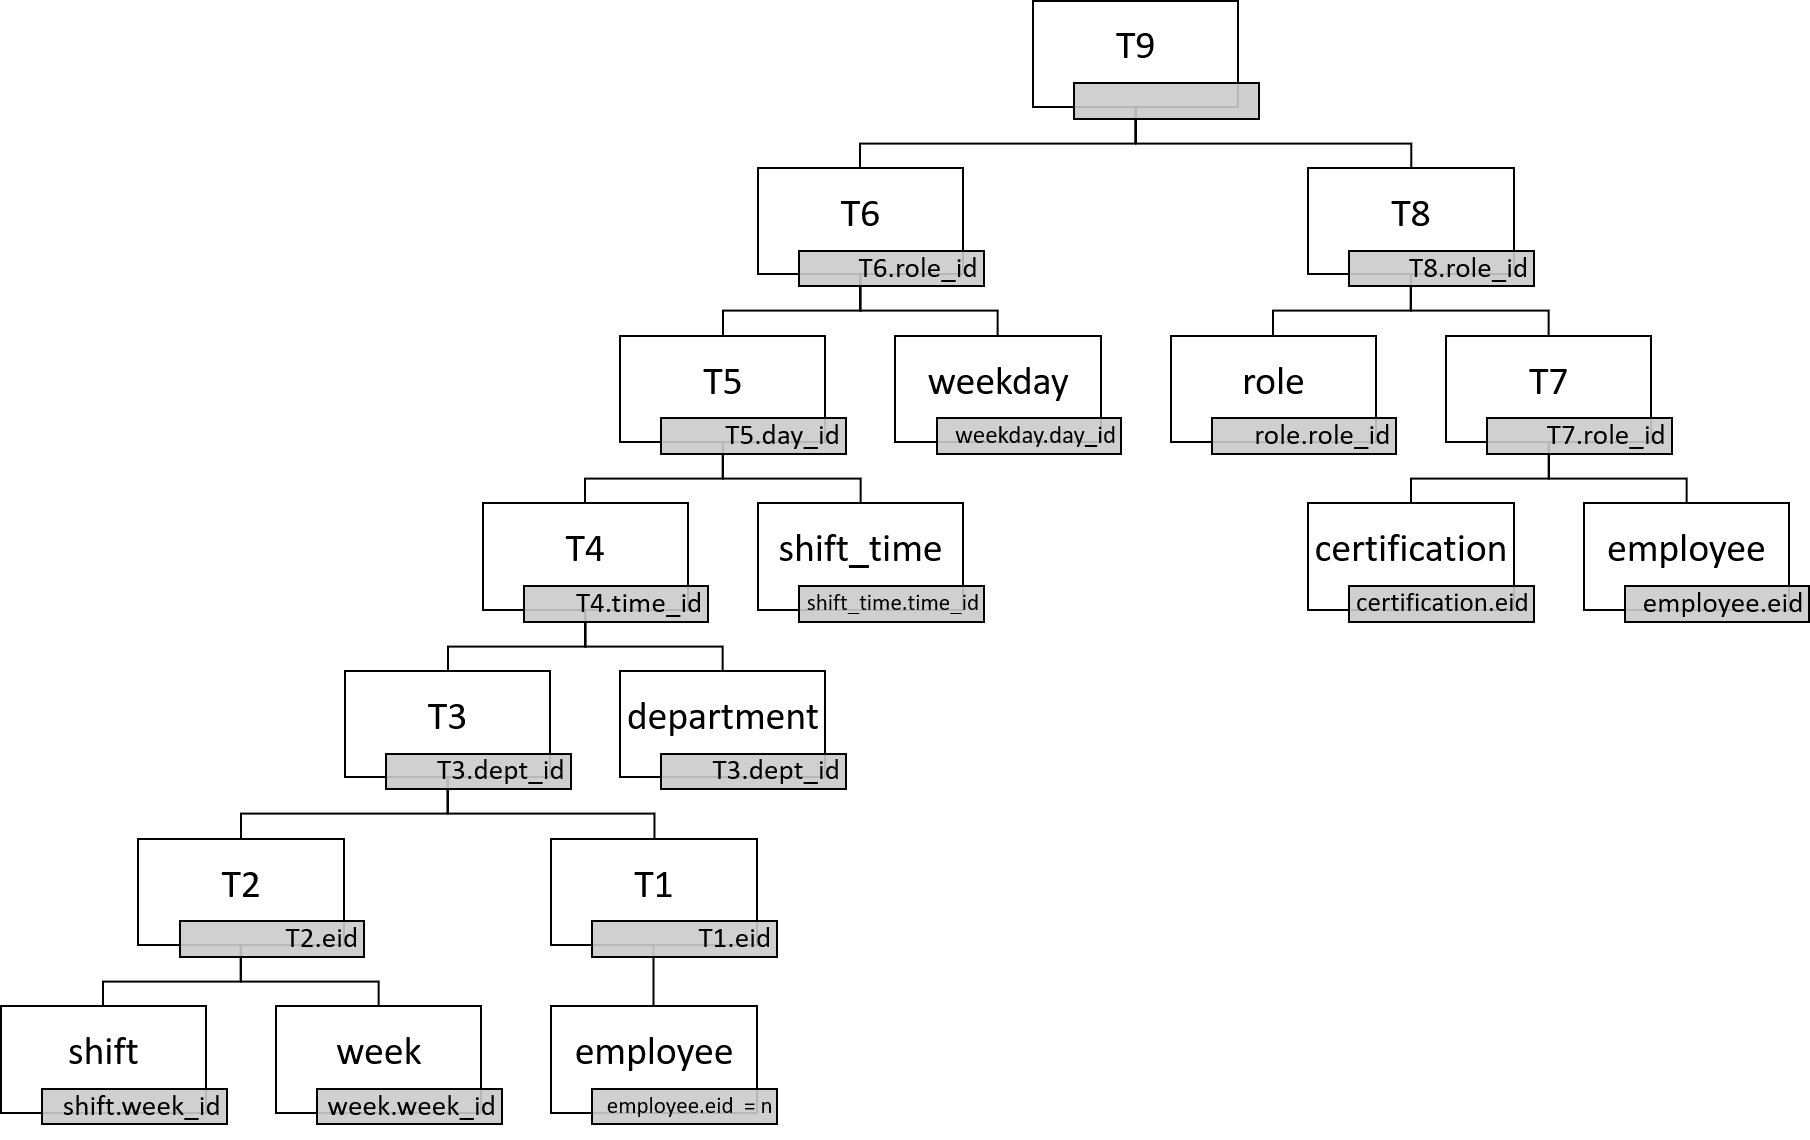
\includegraphics[width=\textwidth]{query1.png}
\end{figure}
On the first query the tables indexed are the shift table on the shift\_id and the employee table on employee\_id. The reason of indexing these tables is because, in comparison to the other tables that are joined in this query, shits and employees have the most rows, and relationships with the fields in other tables. 
\begin{figure}[H]
	\centering
	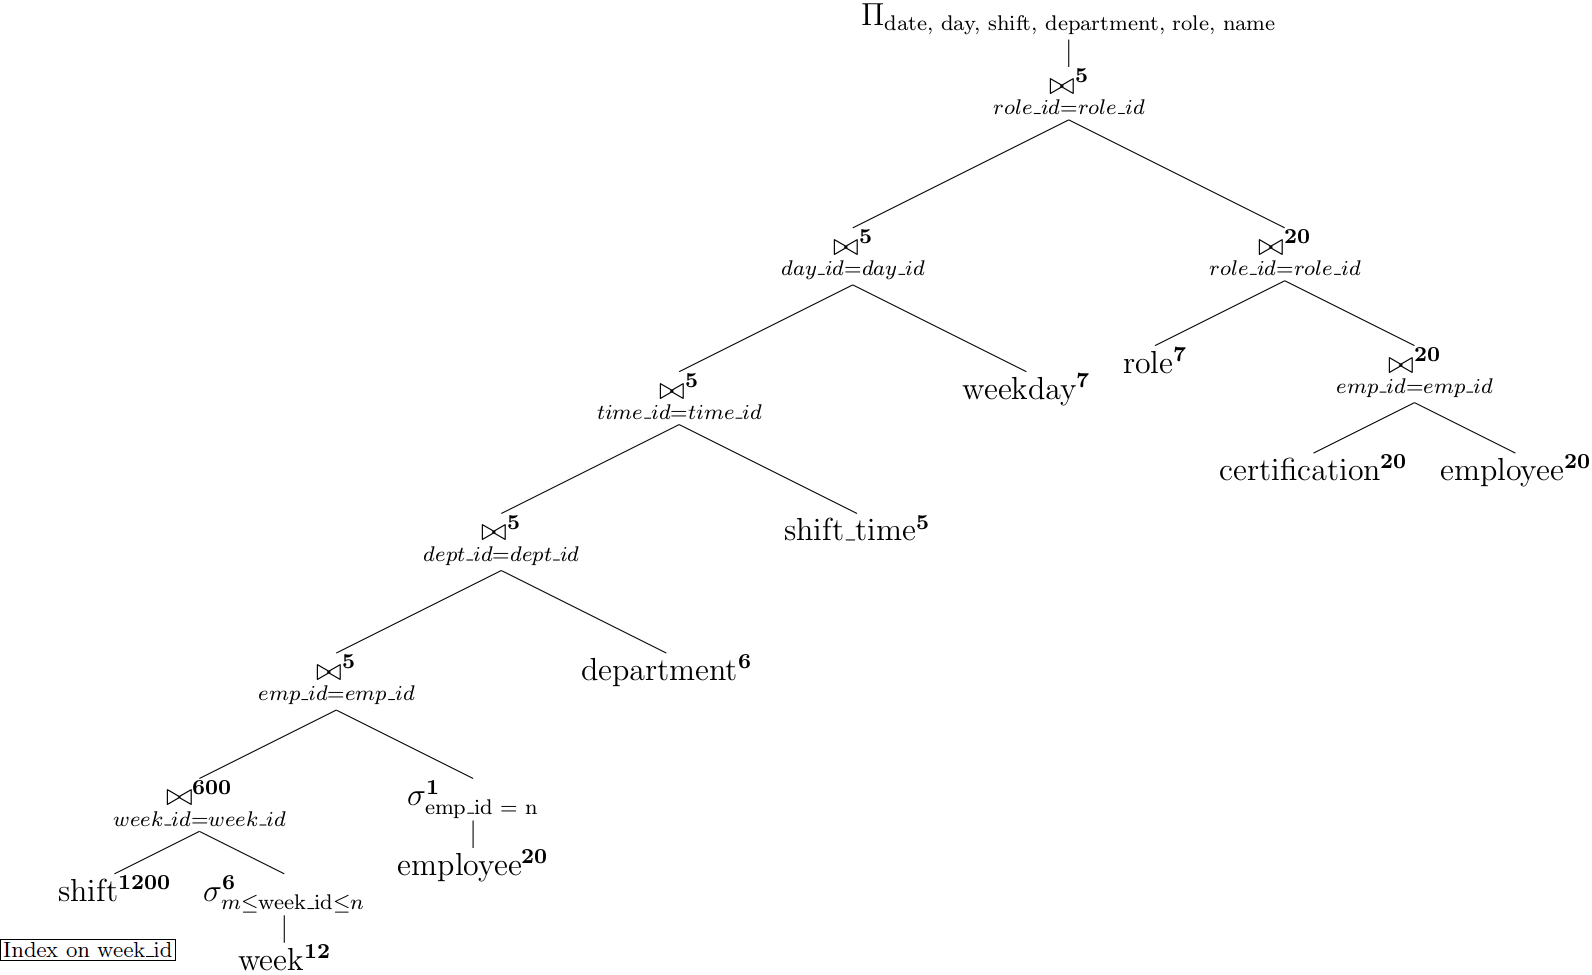
\includegraphics[width=\textwidth]{query1_indexed.png}
\end{figure}
For the first query, indexing employees and shifts tables the access time for each search goes to O(1), instead of the iterative approach of looking at each row and making it O(n), where n is the rows in each table. Indexing in such case is much better because we speedup the process from O(n*m) to O(n) when employees and shifts are combined, where n is the number of employees and m is the number of shifts. Such optimization then has to get added the join of the other tables, but such other tables don't have as many rows and so they won't affect the performance as much as if employees or shifts will not be indexed.
\vspace{1em}
\subsubsection*{Example Data}

\begin{changemargin}{-1.25cm}{-1.25cm}
	\begin{center}
		\lstinputlisting[language=SQL]{./code/query1_data.txt}
	\end{center}
\end{changemargin}


%---------------------------------------------
\subsection*{Query 2}
Query 2 returns a department's need for a single week including the week's start date, day of week, shift start time, shift end time, and needs per role per shift. The query can be tuned by changing the department ID and week ID.

\subsubsection*{MySQL Query}
	\lstinputlisting[language=SQL]{./code/query2.txt}
\begin{figure}[H]
	\centering
	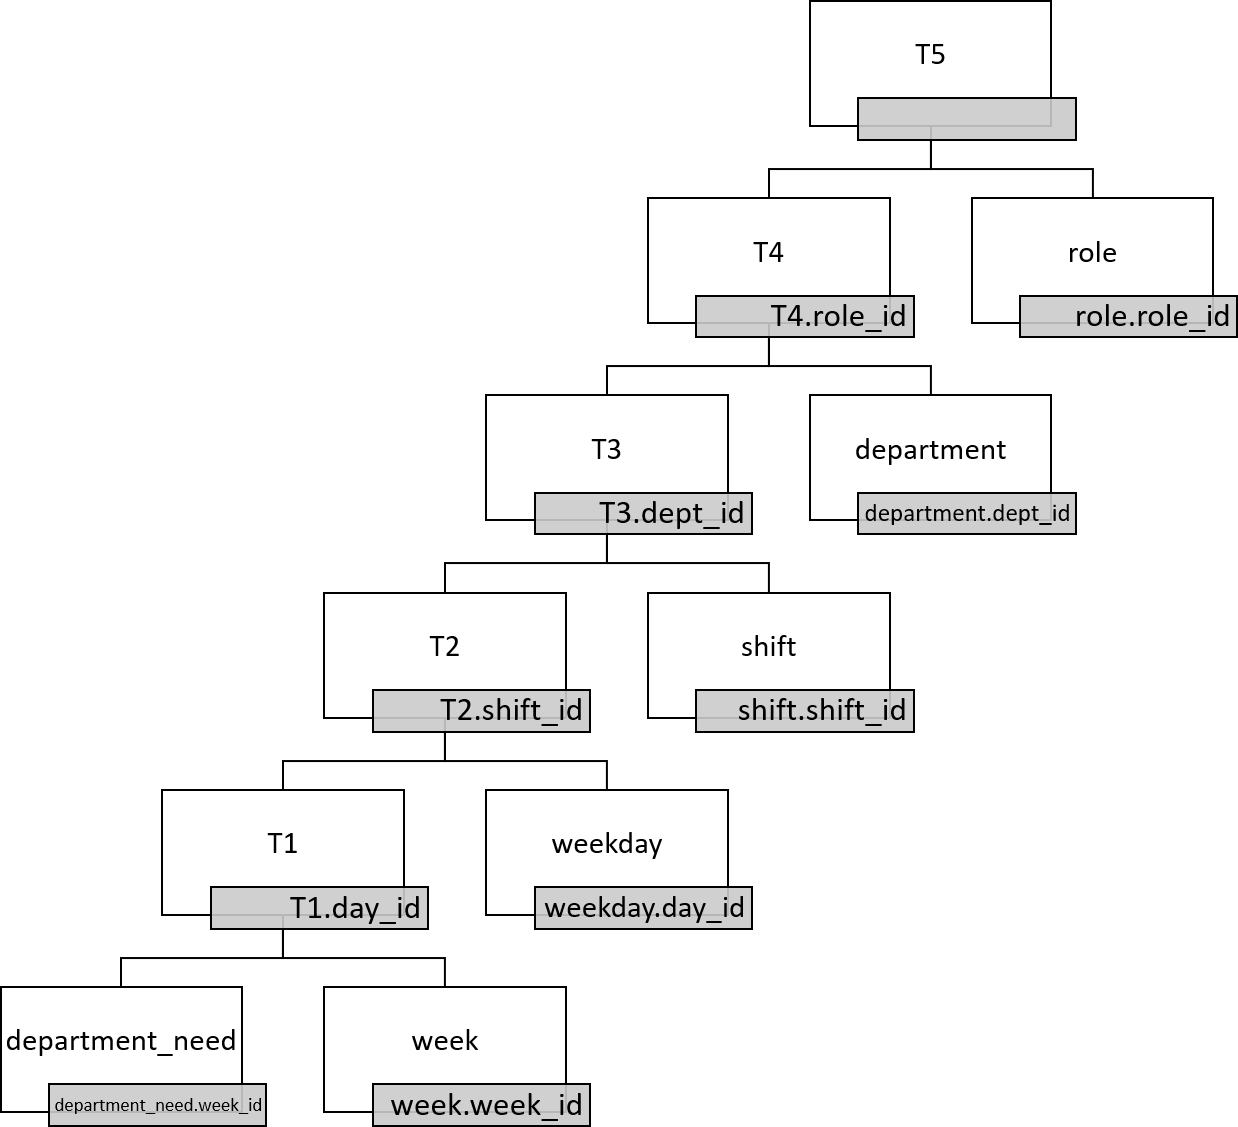
\includegraphics[width=.75\textwidth]{query2.png}
\end{figure}
For the second query the process is much similar to query one. The difference is that the table that is getting joined for the following select query is the departments table. Following the above principle one can optimize the run-time of the query by indexing shifts on shift\_id and department\_id. 
\begin{figure}[H]
	\centering
	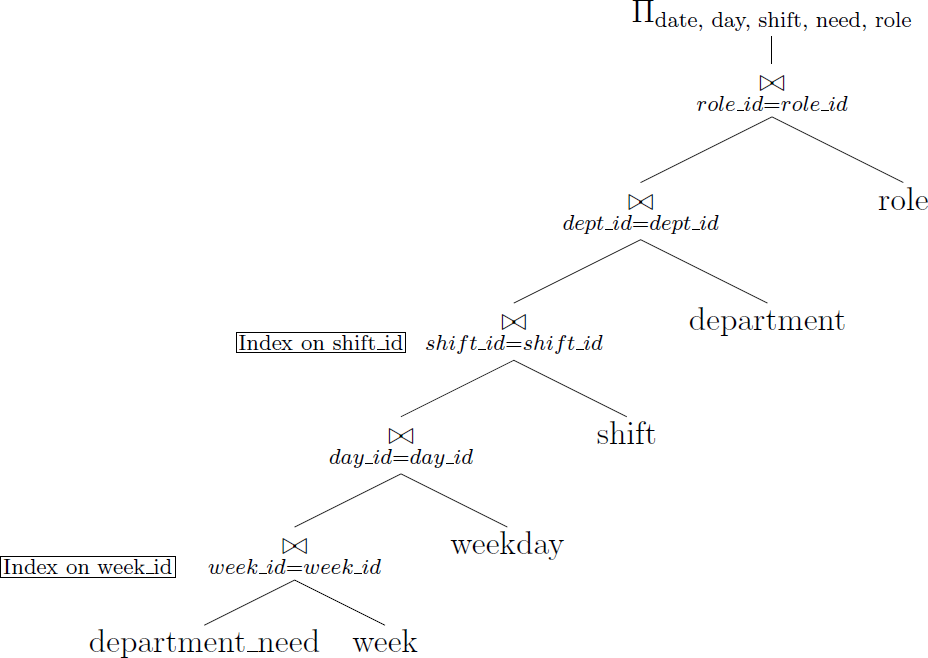
\includegraphics[width=.75\textwidth]{query2_indexed.png}
\end{figure}
Creating the indexing described above yields O(1) access for both shifts and department tables and only giving O(n) for the tables with the least elements and won't affect much the performance.
\vspace{1em}
\subsubsection*{Example Data}
\begin{changemargin}{-1.25cm}{-1.25cm}
	\begin{center}
		\lstinputlisting[language=SQL]{./code/query2_data_truncated.txt}
	\end{center}
\end{changemargin}

%---------------------------------------------
\subsection*{Query 3}
Query 3 will give a single department's schedule for a specified week, ordered by the employee's names. Included information shall contain the start date of the week, the day of the week, shift start and end times, the employee's name, and their phone number. The department and week ID values will need to be changed in order to get the desired data.\subsubsection*{MySQL Query}
	\lstinputlisting[language=SQL]{./code/query3.txt}
\begin{figure}[H]
	\centering
	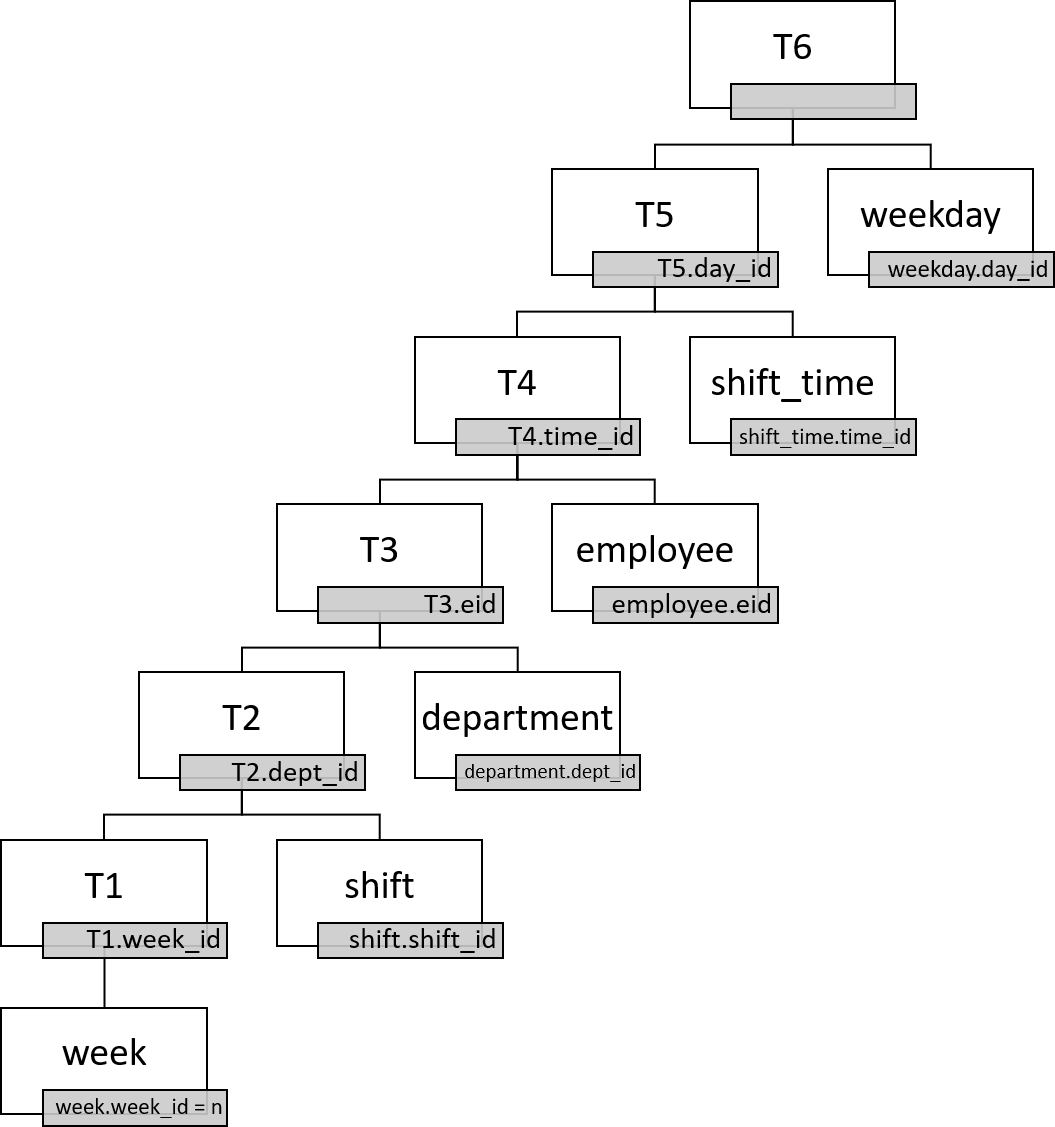
\includegraphics[width=.6\textwidth]{query3.png}
\end{figure}
For the third query a similar index scheme will be implemented on the shift table between the shift.week\_id and week.week\_id. The largest amount of comparisons occur during this table join. 
\begin{figure}[H]
	\centering
	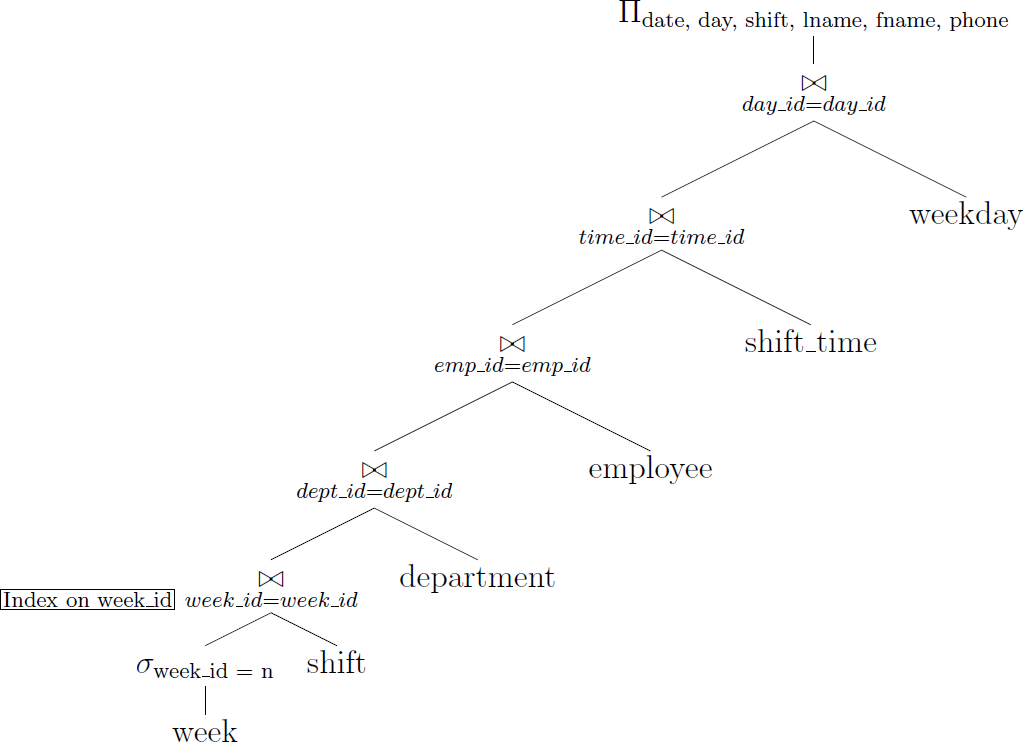
\includegraphics[width=.6\textwidth]{query3_indexed.png}
\end{figure}
The third query would experience the largest speedup in the join between the tables from O(m*n) to O(log(m*n)+c) due to the ability to conduct a binary search on the values corresponding to the correct week ID for both tables and a linear search to find the beginning and end of that week.
\vspace{1em}
\subsubsection*{Example Data}
\begin{changemargin}{-1.25cm}{-1.25cm}
	\begin{center}
		\lstinputlisting[language=SQL]{./code/query3_data.txt}
	\end{center}
\end{changemargin}

%---------------------------------------------
\subsection*{Query 4}
Query 4 will return an employee's pay rate, department, shift start, and shift end times per shift when given a range of dates sorted by date and then shift start time. The total cost per shift shall be calculated by the data parser supplied by you.
\subsubsection*{MySQL Query}
	\lstinputlisting[language=SQL]{./code/query4.txt}
\begin{figure}[H]
	\centering
	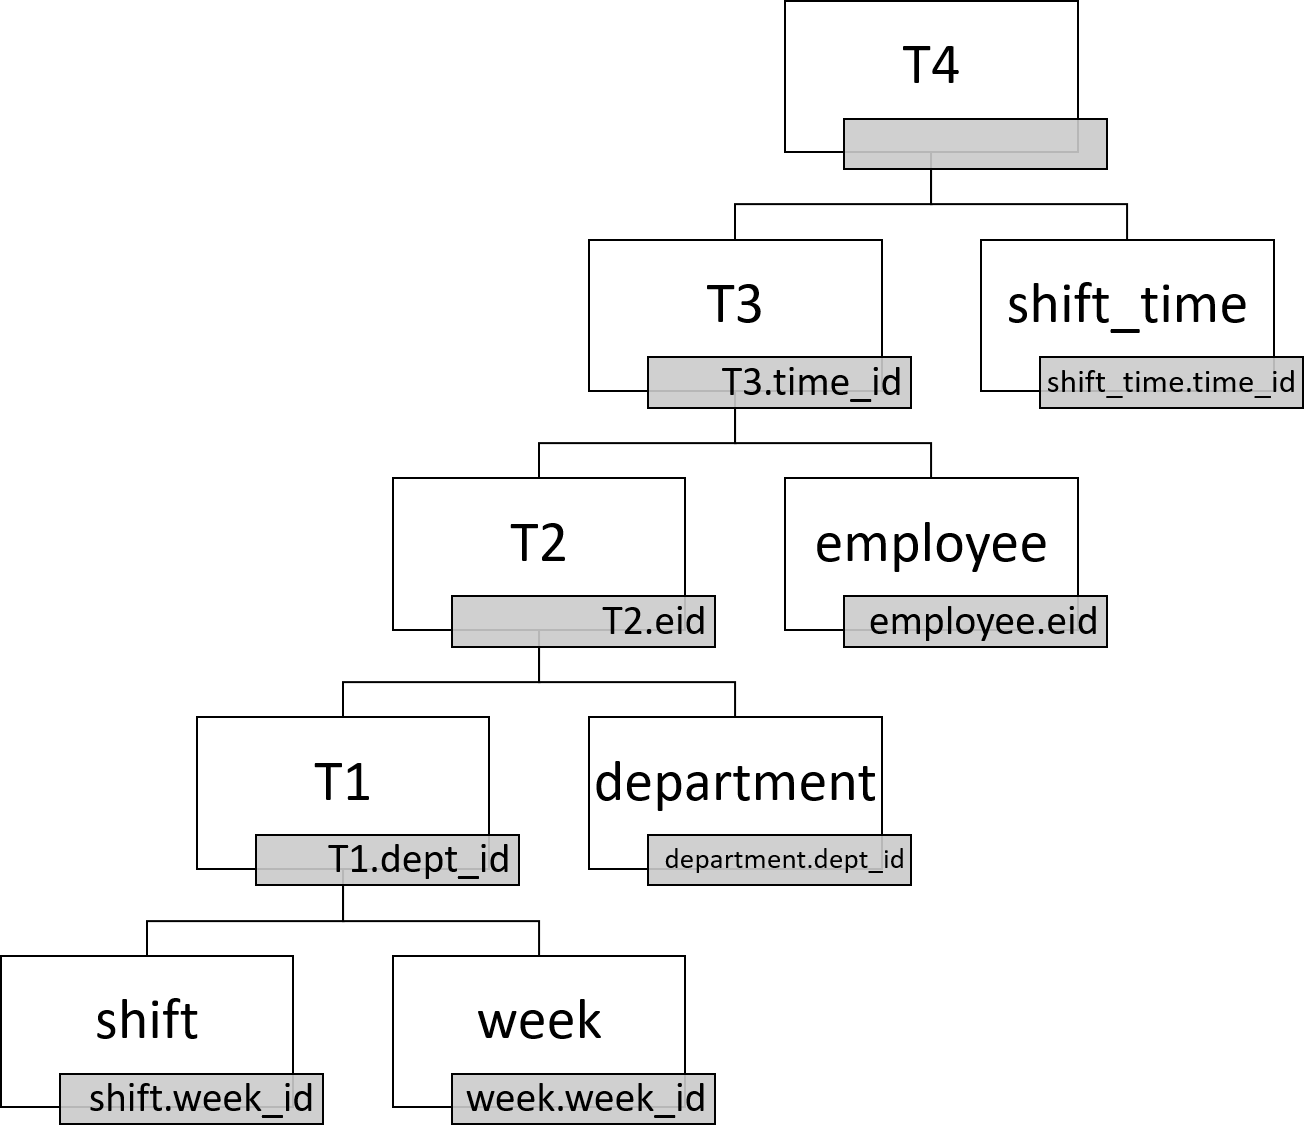
\includegraphics[width=.5\textwidth]{query4.png}
\end{figure}
Query 4 will benefit from the given indexes for a similar reason to Query 3
.\begin{figure}[H]
	\centering
	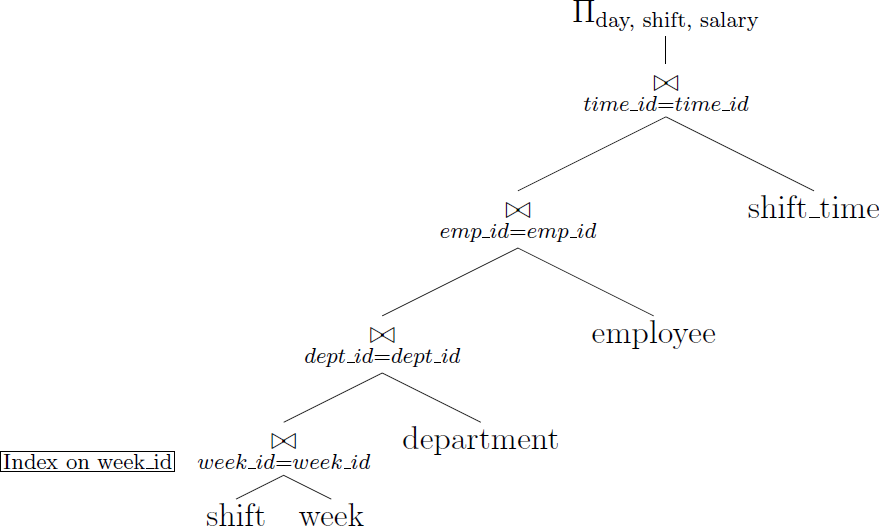
\includegraphics[width=.5\textwidth]{query4_indexed.png}
\end{figure}
On the fourth query the run-time of the tables other than shifts won't be optimized as they aren't the focal point of the select. Thus it will only make sense to index the shifts table on shifts\_id to gain any optimization or performance improvement.  
\vspace{1em}
\subsubsection*{Example Data}
\begin{changemargin}{-1.25cm}{-1.25cm}
	\begin{center}
		\lstinputlisting[language=SQL]{./code/query4_data.txt}
	\end{center}
\end{changemargin}

\section*{Final Notes}
In closing, the supplied data model, table structures, and queries will return the data required by the specification documents. The indexes implemented should provide a considerable performance speedup as the database grows. Output returned by the MySQL queries shall be parse-able by the program supplied by your company in order to create the desired output formats.

\newpage
\section*{Data Model}
\begin{figure}[H]
	\centering
	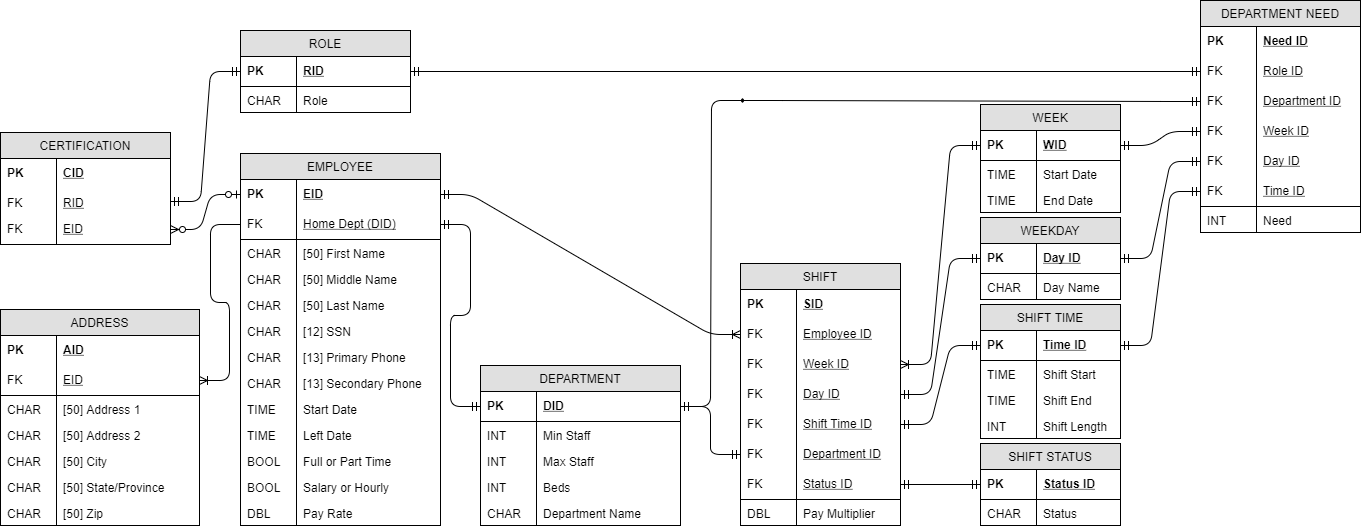
\includegraphics[angle=90, height=\textheight]{er_diag.png}
\end{figure}



%\bigskip{}\decorativeline\bigskip{}
%
%Sincerely,\\
%
%\quad Kyle Salitrik



\end{document}